
\documentclass[letterpaper,hide notes,xcolor={table,svgnames},pdftex]{beamer}
\def\showexamples{t}


%\usepackage[svgnames]{xcolor}

%% Demo talk
%\documentclass[letterpaper,notes=show]{beamer}

\usecolortheme{crane}
\setbeamertemplate{navigation symbols}{}

\usetheme{MyPittsburgh}
%\usetheme{Frankfurt}

%\usepackage{tipa}

\usepackage{hyperref}
\usepackage{graphicx,xspace}
\usepackage[normalem]{ulem}

\newcommand\SF[1]{$\bigstar$\footnote{SF: #1}}



\newcounter{tmpnumSlide}
\newcounter{tmpnumNote}

% old question code
%\newcommand\question[1]{{$\bigstar$ \small \onlySlide{2}{#1}}}
% \newcommand\nquestion[1]{\ifdefined \presentationonly \textcircled{?} \fi \note{\par{\Large \textbf{?}} #1}}
% \newcommand\nanswer[1]{\note{\par{\Large \textbf{A}} #1}}


 \newcommand\mnote[1]{%
   \addtocounter{tmpnumSlide}{1}
   \ifdefined\showcues {~\tiny\fbox{\arabic{tmpnumSlide}}}\fi
   \note{\setlength{\parskip}{1ex}\addtocounter{tmpnumNote}{1}\textbf{\Large \arabic{tmpnumNote}:} {#1\par}}}

\newcommand\mmnote[1]{\note{\setlength{\parskip}{1ex}#1\par}}

%\newcommand\mnote[2][]{\ifdefined\handoutwithnotes {~\tiny\fbox{#1}}\fi
% \note{\setlength{\parskip}{1ex}\textbf{\Large #1:} #2\par}}

%\newcommand\mnote[2][]{{\tiny\fbox{#1}} \note{\setlength{\parskip}{1ex}\textbf{\Large #1:} #2\par}}

\newcommand\mquestion[2]{{~\color{red}\fbox{?}}\note{\setlength{\parskip}{1ex}\par{\Large \textbf{?}} #1} \note{\setlength{\parskip}{1ex}\par{\Large \textbf{A}} #2\par}\ifdefined \presentationonly \pause \fi}

\newcommand\blackboard[1]{%
\ifdefined   \showblackboard
  {#1}
  \else {\begin{center} \fbox{\colorbox{blue!30}{%
         \begin{minipage}{.95\linewidth}%
           \hspace{\stretch{1}} Some space intentionally left blank; done at the blackboard.%
         \end{minipage}}}\end{center}}%
         \fi%
}



%\newcommand\q{\tikz \node[thick,color=black,shape=circle]{?};}
%\newcommand\q{\ifdefined \presentationonly \textcircled{?} \fi}

\usepackage{listings}
\lstset{%
  keywordstyle=\bfseries,
  aboveskip=15pt,
  belowskip=15pt,
  captionpos=b,
  identifierstyle=\ttfamily,
  escapeinside={(*@}{@*)},
  stringstyle=\ttfamiliy,
  frame=lines,
  numbers=left, basicstyle=\scriptsize, numberstyle=\tiny, stepnumber=0, numbersep=2pt}

\usepackage{siunitx}
\newcommand\sius[1]{\num[group-separator = {,}]{#1}\si{\micro\second}}
\newcommand\sims[1]{\num[group-separator = {,}]{#1}\si{\milli\second}}
\newcommand\sins[1]{\num[group-separator = {,}]{#1}\si{\nano\second}}
\sisetup{group-separator = {,}, group-digits = true}

%% -------------------- tikz --------------------
\usepackage{tikz}
\usetikzlibrary{positioning}
\usetikzlibrary{arrows,backgrounds,automata,decorations.shapes,decorations.pathmorphing,decorations.markings,decorations.text}

\tikzstyle{place}=[circle,draw=blue!50,fill=blue!20,thick, inner sep=0pt,minimum size=6mm]
\tikzstyle{transition}=[rectangle,draw=black!50,fill=black!20,thick, inner sep=0pt,minimum size=4mm]

\tikzstyle{block}=[rectangle,draw=black, thick, inner sep=5pt]
\tikzstyle{bullet}=[circle,draw=black, fill=black, thin, inner sep=2pt]

\tikzstyle{pre}=[<-,shorten <=1pt,>=stealth',semithick]
\tikzstyle{post}=[->,shorten >=1pt,>=stealth',semithick]
\tikzstyle{bi}=[<->,shorten >=1pt,shorten <=1pt, >=stealth',semithick]

\tikzstyle{mut}=[-,>=stealth',semithick]

\tikzstyle{treereset}=[dashed,->, shorten >=1pt,>=stealth',thin]

\usepackage{ifmtarg}
\usepackage{xifthen}
\makeatletter
% new counter to now which frame it is within the sequence
\newcounter{multiframecounter}
% initialize buffer for previously used frame title
\gdef\lastframetitle{\textit{undefined}}
% new environment for a multi-frame
\newenvironment{multiframe}[1][]{%
\ifthenelse{\isempty{#1}}{%
% if no frame title was set via optional parameter,
% only increase sequence counter by 1
\addtocounter{multiframecounter}{1}%
}{%
% new frame title has been provided, thus
% reset sequence counter to 1 and buffer frame title for later use
\setcounter{multiframecounter}{1}%
\gdef\lastframetitle{#1}%
}%
% start conventional frame environment and
% automatically set frame title followed by sequence counter
\begin{frame}%
\frametitle{\lastframetitle~{\normalfont(\arabic{multiframecounter})}}%
}{%
\end{frame}%
}
\makeatother

\makeatletter
\newdimen\tu@tmpa%
\newdimen\ydiffl%
\newdimen\xdiffl%
\newcommand\ydiff[2]{%
    \coordinate (tmpnamea) at (#1);%
    \coordinate (tmpnameb) at (#2);%
    \pgfextracty{\tu@tmpa}{\pgfpointanchor{tmpnamea}{center}}%
    \pgfextracty{\ydiffl}{\pgfpointanchor{tmpnameb}{center}}%
    \advance\ydiffl by -\tu@tmpa%
}
\newcommand\xdiff[2]{%
    \coordinate (tmpnamea) at (#1);%
    \coordinate (tmpnameb) at (#2);%
    \pgfextractx{\tu@tmpa}{\pgfpointanchor{tmpnamea}{center}}%
    \pgfextractx{\xdiffl}{\pgfpointanchor{tmpnameb}{center}}%
    \advance\xdiffl by -\tu@tmpa%
}
\makeatother
\newcommand{\copyrightbox}[3][r]{%
\begin{tikzpicture}%
\node[inner sep=0pt,minimum size=2em](ciimage){#2};
\usefont{OT1}{phv}{n}{n}\fontsize{4}{4}\selectfont
\ydiff{ciimage.south}{ciimage.north}
\xdiff{ciimage.west}{ciimage.east}
\ifthenelse{\equal{#1}{r}}{%
\node[inner sep=0pt,right=1ex of ciimage.south east,anchor=north west,rotate=90]%
{\raggedleft\color{black!50}\parbox{\the\ydiffl}{\raggedright{}#3}};%
}{%
\ifthenelse{\equal{#1}{l}}{%
\node[inner sep=0pt,right=1ex of ciimage.south west,anchor=south west,rotate=90]%
{\raggedleft\color{black!50}\parbox{\the\ydiffl}{\raggedright{}#3}};%
}{%
\node[inner sep=0pt,below=1ex of ciimage.south west,anchor=north west]%
{\raggedleft\color{black!50}\parbox{\the\xdiffl}{\raggedright{}#3}};%
}
}
\end{tikzpicture}
}


%% --------------------

%\usepackage[excludeor]{everyhook}
%\PushPreHook{par}{\setbox0=\lastbox\llap{MUH}}\box0}

%\vspace*{\stretch{1}

%\setbox0=\lastbox \llap{\textbullet\enskip}\box0}

\setlength{\parskip}{\fill}

\newcommand\noskips{\setlength{\parskip}{1ex}}
\newcommand\doskips{\setlength{\parskip}{\fill}}

\newcommand\xx{\par\vspace*{\stretch{1}}\par}
\newcommand\xxs{\par\vspace*{2ex}\par}
\newcommand\tuple[1]{\langle #1 \rangle}
\newcommand\code[1]{{\sf \footnotesize #1}}
\newcommand\ex[1]{\uline{Example:} \ifdefined \presentationonly \pause \fi
  \ifdefined\showexamples#1\xspace\else{\uline{\hspace*{2cm}}}\fi}

\newcommand\ceil[1]{\lceil #1 \rceil}


\AtBeginSection[]
{
   \begin{frame}
       \frametitle{Outline}
       \tableofcontents[currentsection]
   \end{frame}
}



\pgfdeclarelayer{edgelayer}
\pgfdeclarelayer{nodelayer}
\pgfsetlayers{edgelayer,nodelayer,main}

\tikzstyle{none}=[inner sep=0pt]
\tikzstyle{rn}=[circle,fill=Red,draw=Black,line width=0.8 pt]
\tikzstyle{gn}=[circle,fill=Lime,draw=Black,line width=0.8 pt]
\tikzstyle{yn}=[circle,fill=Yellow,draw=Black,line width=0.8 pt]
\tikzstyle{empty}=[circle,fill=White,draw=Black]
\tikzstyle{bw} = [rectangle, draw, fill=blue!20, 
    text width=4em, text centered, rounded corners, minimum height=2em]
    
    \newcommand{\CcNote}[1]{% longname
	This work is licensed under the \textit{Creative Commons #1 3.0 License}.%
}
\newcommand{\CcImageBy}[1]{%
	\includegraphics[scale=#1]{creative_commons/cc_by_30.pdf}%
}
\newcommand{\CcImageSa}[1]{%
	\includegraphics[scale=#1]{creative_commons/cc_sa_30.pdf}%
}
\newcommand{\CcImageNc}[1]{%
	\includegraphics[scale=#1]{creative_commons/cc_nc_30.pdf}%
}
\newcommand{\CcGroupBySa}[2]{% zoom, gap
	\CcImageBy{#1}\hspace*{#2}\CcImageNc{#1}\hspace*{#2}\CcImageSa{#1}%
}
\newcommand{\CcLongnameByNcSa}{Attribution-NonCommercial-ShareAlike}

\newenvironment{changemargin}[1]{% 
  \begin{list}{}{% 
    \setlength{\topsep}{0pt}% 
    \setlength{\leftmargin}{#1}% 
    \setlength{\rightmargin}{1em}
    \setlength{\listparindent}{\parindent}% 
    \setlength{\itemindent}{\parindent}% 
    \setlength{\parsep}{\parskip}% 
  }% 
  \item[]}{\end{list}} 



\usepackage{tikz-3dplot}

\title{Lecture 35 --- Library Card}

\author{Jeff Zarnett \\ \small \texttt{jzarnett@uwaterloo.ca}}
\institute{Department of Electrical and Computer Engineering \\
  University of Waterloo}
\date{\today}

\begin{document}

\begin{frame}
  \titlepage
\end{frame}


\begin{frame}
\frametitle{Library Card}
\begin{changemargin}{1cm}
Some advanced engineering design concepts.

Book one: \emph{The Mythical Man-Month}.

Book two: \emph{The Logic of Failure}. \mnote{A book about how to deal with systems with complex interactions.}

Book three: \emph{The Human Factor}. \mnote{how to design systems for humans.}

\end{changemargin}
\end{frame}

\part{The Mythical Man-Month}
\frame{\partpage}

\begin{frame}
\frametitle{The Mythical Man-Month}
\begin{changemargin}{1cm}

Sometimes during development, you might discover that your project is behind or buggy. 

Management might attempt to solve this by adding more resources (workers) to the project.
\end{changemargin}
\end{frame}

\begin{frame}
\frametitle{The Mythical Man-Month}
\begin{changemargin}{0.1cm}

\begin{quote}
	\textit{Adding manpower to a late software project makes it later.}
\end{quote}
\end{changemargin}
\end{frame}

\begin{frame}
\frametitle{The Mythical Man-Month}
\begin{changemargin}{1cm}
Estimates are difficult to make and usually optimistic.

Our estimating techniques confuse effort with progress.\\
We assume programmers and monte are interchangeable. 

When a schedule slip is recognized, the natural tendency is to add more programmers. 

It makes the problem worse! 
\end{changemargin}
\end{frame}

\begin{frame}
\frametitle{The Mythical Man-Month}
\begin{changemargin}{1cm}
A \alert{man-month} is defined as the amount of work one programmer can accomplish in one calendar month. 

Cost varies by programmers and months, but progress doesn't. 

It is therefore dangerous and wrong to try to measure a programming task using this unit.
\end{changemargin}
\end{frame}

\begin{frame}
\frametitle{The Mythical Man-Month}
\begin{changemargin}{1cm}
Workers and time can be traded off against one another only if there is no communication required between workers. 

(Does this sound familiar?) 

When more programmers are added, we have to consider training and intercommunication.
\end{changemargin}
\end{frame}

\begin{frame}
\frametitle{The Mythical Man-Month: Training}
\begin{changemargin}{1cm}
Training scales linearly ($n$) with the number of people. 

Training consists of bringing a new programmer up to speed on the project and its related technology. 

This is a one-time cost when someone joins a project. 

A new programmer, no matter how intelligent, is not fully productive immediately.
\end{changemargin}
\end{frame}

\begin{frame}
\frametitle{The Mythical Man-Month: Intercommunication}
\begin{changemargin}{1cm}

Intercommunication scales at $n (n - 1) / 2$. \\
\quad if each part of the task is separately co-ordinated.

3 workers require 3x as much intercommunication as 2.

4 require 6 times as much as 2. 

\end{changemargin}
\end{frame}

\begin{frame}
\frametitle{The Mythical Man-Month: Intercommunication}
\begin{changemargin}{1cm}
Adding a programmer increases the communication costs.

This cost can outweigh the benefit the programmer brings.

Thus, the project gets later.
\end{changemargin}
\end{frame}


\begin{frame}
\frametitle{The Mythical Man-Month: Example}
\begin{changemargin}{1cm}
Suppose a task is estimated at 12 man-months.

It is divided up such that three are three programmers who will work for four months. 

Milestones A, B, C, and D, 1 at the end of each month. 

\end{changemargin}
\end{frame}

\begin{frame}
\frametitle{The Mythical Man-Month: Example}
\begin{changemargin}{1cm}
A delay occurs and milestone A isn't completed in 1 month.


They assume that only milestone A is incorrect and 9 man-months of work remain, and two months remain. 

So 4.5 programmers will be needed. 

Hire two programmers. 
\end{changemargin}
\end{frame}

\begin{frame}
\frametitle{The Mythical Man-Month: Example}
\begin{changemargin}{1cm}
Assume it takes 1 month to train these 2 new programmers.

Developer time is consumed by training the new people.

Tasks must be re-partitioned and re-assigned.

Integration testing increases.

\end{changemargin}
\end{frame}

\begin{frame}
\frametitle{The Mythical Man-Month: Example}
\begin{changemargin}{1cm}
At the end of the third month, we would still have more than 7 man-months of work to do and five trained programmers. 

The project is still late! 

The temptation is to then add yet more people, but this makes things worse, not better. 

\end{changemargin}
\end{frame}

\begin{frame}
\frametitle{No Silver Bullet}
\begin{changemargin}{1cm}
\begin{quote}
\textit{There is no single development, in either technology or in management technique, that by itself promises even one order-of-magnitude improvement in productivity, in reliability, in simplicity.}
\end{quote}

\end{changemargin}
\end{frame}

\begin{frame}
\frametitle{No Silver Bullet}
\begin{changemargin}{1cm}
The term ``silver bullet'' comes from the werewolf folklore.

Werewolves can be stopped by being shot with a silver bullet.

A metaphor meaning a straightforward, simple solution to what is otherwise a complex problem. 

\end{changemargin}
\end{frame}

\begin{frame}
\frametitle{No Silver Bullet}
\begin{changemargin}{1cm}
Example: diet books. 

Promise something simple as the solution to weight loss.

``Eat Goji Berries!'' 

It is, unfortunately, not that simple. 

\end{changemargin}
\end{frame}


\begin{frame}
\frametitle{No Silver Bullet}
\begin{changemargin}{1cm}
It is unlikely that we will ever find a silver bullet.

There are probably no inventions that will do for software development what electronics did for computer hardware. 

The hard part of building software is not the accidental complexity, but the essential complexity.

The hard part is the specification and design of testing the concepts, not the work of implementing it. 

\end{changemargin}
\end{frame}

\begin{frame}
\frametitle{No Silver Bullet: Complexity}
\begin{changemargin}{1cm}

Software is very complex, and this is an essential property. 

In physics we have simplified models for complex phenomena. \\
\quad (e.g., Newton's equations). 

Complexities (like relativity) can be ignored. 

In software, the details, are the essential parts and cannot be abstracted away. 
\end{changemargin}
\end{frame}

\begin{frame}
\frametitle{No Silver Bullet: Complexity}
\begin{changemargin}{1cm}
Much of the complexity is arbitrary. 

It must conform to other software or hardware, designed by imperfect humans. 

Your software has to run on Windows, and has to conform to all the details and oddities of Windows...

\end{changemargin}
\end{frame}

\begin{frame}
\frametitle{No Silver Bullet: Changeability}
\begin{changemargin}{1cm}
Software is much more changeable than physical objects. 

Cars and buildings get upgrades infrequently, if ever. 

If Ford comes up with a better version of a car, that goes into next year's model. 

Software is changeable because it is not a physical artifact. 

\end{changemargin}
\end{frame}

\begin{frame}
\frametitle{No Silver Bullet: Changeability}
\begin{changemargin}{1cm}
The fact that the cost of changing a building is high discourages arbitrary changes. 

Successful software is changed because users want to: 
\begin{itemize}
	\item apply it to new problems; or 
	\item adapt it to new hardware or operating systems.
\end{itemize}

\end{changemargin}
\end{frame}

\begin{frame}
\frametitle{No Silver Bullet: Tools}
\begin{changemargin}{1cm}
Our tools have improved to make attacking some of this complexity better, but none alone is the magic solution: 
\begin{itemize}
	\item high-level languages
	\item integrated development environments
	\item object-oriented programming
	\item verification
\end{itemize}

\end{changemargin}
\end{frame}


\begin{frame}
\frametitle{No Silver Bullet: Tools}
\begin{changemargin}{1cm}
 breakthroughs have been promised for a long time, but never seem to come through:
 
\begin{itemize}
	\item artificial intelligence
	\item automatic programming
	\item graphical programming
\end{itemize}

Maybe these will arrive at some point.

\end{changemargin}
\end{frame}

\begin{frame}
\frametitle{No Silver Bullet: Solution}
\begin{changemargin}{1cm}

The most powerful tool we have is to have great developers.

(Which is why you are in this class.)
\end{changemargin}
\end{frame}


\part{The Logic of Failure}
\frame{\partpage}

\begin{frame}
\frametitle{The Logic of Failure}
\begin{changemargin}{1cm}
\alert{Tanaland} is a fictional region in West Africa.

Used for a simulation.

Participants in the study get dictatorial power.

Goal: improve the inhabitants' lives over 10 years. 

\end{changemargin}
\end{frame}


\begin{frame}
\frametitle{The Logic of Failure: Tanaland}
\begin{changemargin}{1cm}

Fields are not very productive, partly because of the rodents.

The obvious solution is to exterminate the pests. 

At first, this results in an increase in the fields' productivity.

\end{changemargin}
\end{frame}


\begin{frame}
\frametitle{The Logic of Failure: Tanaland}
\begin{changemargin}{1cm}

Then, insect populations increase (they feed on the fields).

Larger predators begin attacking the cattle.\\
\quad There are no longer the mice and rats to feed on.

Eliminating the rodents in the end has no effect\\ 
\quad or it may have actually made the situation worse. 

\end{changemargin}
\end{frame}

\begin{frame}
\frametitle{The Logic of Failure: Tanaland}
\begin{changemargin}{1cm}

The critical insight from the simulations:\\
\quad We cannot do any one thing in isolation. 

Any change has multiple effects.

Some of them unpredictable.

\end{changemargin}
\end{frame}

\begin{frame}
\frametitle{The Logic of Failure: Definitions}
\begin{changemargin}{1cm}
\alert{Positive Feedback}: an increase in a variable produces a further increase in that variable.

A decrease produces a further decrease.

Example: Rabbit population (in isolation).

\end{changemargin}
\end{frame}

\begin{frame}
\frametitle{The Logic of Failure: Definitions}
\begin{changemargin}{1cm}
\alert{Negative Feedback}: an increase in one variable produces a decrease in another and vice versa.

This maintains equilibrium.

Example: Predator-Prey System.

\end{changemargin}
\end{frame}

\begin{frame}
\frametitle{The Logic of Failure: Definitions}
\begin{changemargin}{1cm}
\alert{Well-Buffered System}: has many variables regulated by negative feedback.

It can absorb many disturbances without becoming unstable. 

However, buffers are limited and may eventually be exhausted. 

Predators can hunt the prey to extinction.

\end{changemargin}
\end{frame}

\begin{frame}
\frametitle{The Logic of Failure: Definitions}
\begin{changemargin}{1cm}
\alert{Critical Variables}: interact with many other variables.

Altering one has a major impact on the state of the system.

\end{changemargin}
\end{frame}

\begin{frame}
\frametitle{The Logic of Failure: Definitions}
\begin{changemargin}{1cm}
\alert{Indicator Variables}: depend on many other variables.

Exert very little influence themselves.

Help understanding of the current status of the system. 

\end{changemargin}
\end{frame}


\begin{frame}
\frametitle{The Logic of Failure: Conflicting Goals}
\begin{changemargin}{1cm}
We can rarely focus on one goal at a time.

Analysis shows that shopping options and transportation links in a suburb are inadequate.

We can choose to improve one of these.

Choosing one will have an impact on the other.

\end{changemargin}
\end{frame}

\begin{frame}
\frametitle{The Logic of Failure: Conflicting Goals}
\begin{changemargin}{1cm}
Improve transportation, and people might shop in the city. \\
\quad Depriving local shops of revenue.


Or people from the city will come shop in the suburbs.

If we improve local shopping opportunities, people will shop locally and things will improve for local businesses. 

\end{changemargin}
\end{frame}

\begin{frame}
\frametitle{The Logic of Failure: Conflicting Goals}
\begin{changemargin}{1cm}
By solving problem $X$ we create problem $Y$. 

If the appearance of $Y$ is not immediate, it might not be obvious that solving $X$ was the cause. 

Solving $Y$ could very well result in a recurrence of $X$. 

The cycle begins again.

Example: headache and stomachache.

\end{changemargin}
\end{frame}

\begin{frame}
\frametitle{The Logic of Failure: Back to Tanaland}
\begin{changemargin}{1cm}
Let's try to help some inhabitants of Tanaland, the Moros. 

Normal strategy: solve one problem at a time.  

Most people start with combating the Tsetse fly.

The next most likely: drill wells to alleviate a water shortage.
\end{changemargin}
\end{frame}

\begin{frame}
\frametitle{The Logic of Failure: Back to Tanaland}
\begin{changemargin}{1cm}

Cattle live longer and the water shortage is eased.\\
\quad They can have bigger fields of grass and more cattle. 

They can sell some grain and cattle.

The next step most people take is to address medical care.\\
\quad Infant mortality declines and life expectancy increases. 

This results in an increase in population. 

This can go three ways, but all end in the same (grim) way.


\end{changemargin}
\end{frame}

\begin{frame}
\frametitle{The Logic of Failure: Tanaland Scenario 1}
\begin{changemargin}{1cm}

Number of cattle exceeds the carrying capacity of the fields. 

The cattle are not only eating the grass, but tearing it up. 

The vegetated area is overgrazed and shrinks. 

The smaller the amount of grass, the more desperate the hunger of the cattle, and the more they damage the grass. 


\end{changemargin}
\end{frame}

\begin{frame}
\frametitle{The Logic of Failure: Tanaland Scenario 1}
\begin{changemargin}{1cm}

There is a solution  -- slaughter or sell the majority of the cows.
 
Seems like a ``radical'' step and people are reluctant to do it. 
 
Once the grass is gone: the cattle will die, the Moros will be short of food, and they will starve.

\end{changemargin}
\end{frame}


\begin{frame}
\frametitle{The Logic of Failure: Tanaland Scenario 1}
\begin{center}
	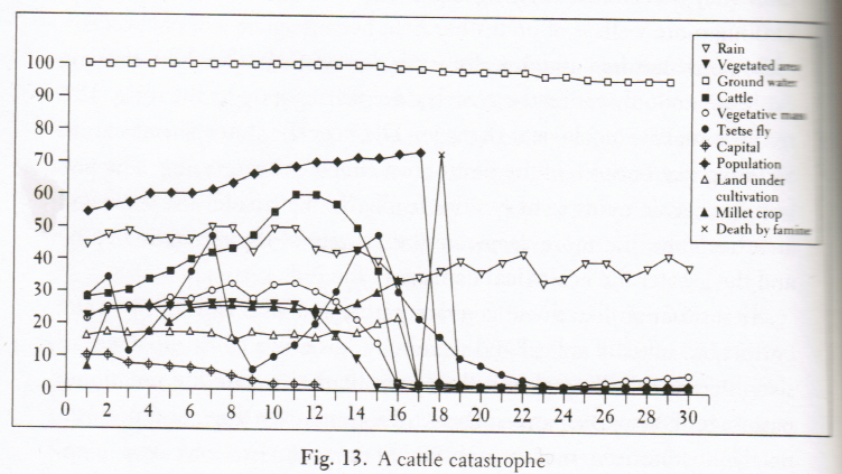
\includegraphics[width=0.8\textwidth]{images/cattlecatastrophe.png}
\end{center}
\end{frame}


\begin{frame}
\frametitle{The Logic of Failure: Tanaland Scenario 2}
\begin{changemargin}{1cm}

If cattle and human populations are kept in check, the system might seem stable for some time.

At some point, however, the wells start yielding less water.

 The obvious solution is to drill more wells.
 
 Might write it off as a temporary problem.
 
\end{changemargin}
\end{frame}

\begin{frame}
\frametitle{The Logic of Failure: Tanaland Scenario 2}
\begin{changemargin}{1cm}
Groundwater supply is being depleted.

Drilling wells to solve depleted wells is positive feedback.

More wells = faster depletion.


\end{changemargin}
\end{frame}

\begin{frame}
\frametitle{The Logic of Failure: Tanaland Scenario 2}
\begin{changemargin}{1cm}
Shortage of water means no irrigation of the grass.

Cattle start overgrazing, then die.

Then Moros are short of food and starve.

Just like scenario 1.

\end{changemargin}
\end{frame}

\begin{frame}
\frametitle{The Logic of Failure: Tanaland Scenario 3}
\begin{changemargin}{1cm}
Another participant just focused on healthcare.

Infant mortality decreased, life expectancy increased.

The population grows: more requirement for food and water.

If nothing is done, people will starve.

Attempts to fix it can turn into Scenario 1 or 2.

\end{changemargin}
\end{frame}

\begin{frame}
\frametitle{The Logic of Failure: Tanaland Conclusions}
\begin{changemargin}{1cm}
Participants dealt with things as independent mini-systems.\\
\quad Not a single, complex, interrelated system. 

They focus on the problem at hand. \\
\quad Not what the consequences are or could be. 

Future problems don't seem important.

Cause-effect relationships are unclear.\\
\quad At best, revealed by experimentation.

\end{changemargin}
\end{frame}


\begin{frame}
\frametitle{The Logic of Failure: Lessons Learned}
\begin{changemargin}{1cm}
Good participants asked why-questions, not what-questions.

More interested in how the events were interrelated.

People who did poorly tended to take events at face value.

\end{changemargin}
\end{frame}


\begin{frame}
\frametitle{The Logic of Failure: Tips}
\begin{changemargin}{1cm}
 Some tips for dealing with complex systems:
 
\begin{itemize}
	\item State goals clearly.
	\item Recognize that it's not always possible to accomplish all our goals at once (goals may conflict).
	\item Establish priorities and change them when circumstances require.
\end{itemize}

\end{changemargin}
\end{frame}


\begin{frame}
\frametitle{The Logic of Failure: Tips}
\begin{changemargin}{1cm}
 Some tips for dealing with complex systems:
 
\begin{itemize}
	\item Learn a model of the system and use it to predict likely outcomes.
	\item Gather information at an appropriate level: neither too much nor too little.
	\item Know when to gather more information and when enough. 
	\item Avoid excessive abstraction.
\end{itemize}

\end{changemargin}
\end{frame}

\begin{frame}
\frametitle{The Logic of Failure: Tips}
\begin{changemargin}{1cm}
 Some tips for dealing with complex systems:
 
\begin{itemize}
	\item Don't hastily blame all events on one central cause.
	\item Avoid ``knee-jerk'' reactions.
	\item Analyze errors and learn from them.
\end{itemize}

\end{changemargin}
\end{frame}

\part{The Human Factor}
\frame{\partpage}

\begin{frame}
\frametitle{The Human Factor: Mercedes E320}
\begin{changemargin}{1cm}
In the Mercedes-Benz E320, drivers can check the oil electronically from the driver's seat. 

Old, manual procedure:
\begin{enumerate}
	\item Turn the car off.
	\item Wait for the oil to settle.
	\item Open the hood.
	\item Find a rag to wipe the dipstick.
	\item Identify the dipstick.
	\item Wipe it.
	\item Reinsert it.
	\item Extract it.
	\item Read it.
\end{enumerate}
\end{changemargin}
\end{frame}

\begin{frame}
\frametitle{The Human Factor: Mercedes E320}
\begin{changemargin}{1cm}
New procedure in the E320.
\begin{enumerate}
	\item Turn the car off.
	\item Wait for the oil to settle.
	\item Turn the ignition two notches to the right.
	\item Wait five seconds.
	\item Press the odometer reset button twice.
\end{enumerate}
\end{changemargin}
\end{frame}

\begin{frame}
\frametitle{The Human Factor: Mercedes E320}
\begin{changemargin}{1cm}
Will users remember these set of steps? Probably not. 

Most people will just perform the manual procedure. 

Designers didn't deliberately build this system to be complicated and unintuitive.

\end{changemargin}
\end{frame}

\begin{frame}
\frametitle{The Human Factor: Designers}
\begin{changemargin}{1cm}
Designers are responsible for this.

Tech people like playing with gadgets and figuring out the cool features of something.

Most people just want to use the thing.

Most users are not like designers.

\end{changemargin}
\end{frame}

\begin{frame}
\frametitle{The Human Factor: BMW iDrive}
\begin{changemargin}{1cm}
The 2003 BMW 7 series had an ``iDrive'' system.

iDrive has between 700 and 800 features.

\end{changemargin}
\end{frame}

\begin{frame}
\frametitle{The Human Factor: BMW iDrive}
\begin{changemargin}{1cm}
\begin{quote}
\textit{It reminds me of software designers who become so familiar with the workings of their products that they forget actual customers at some point will have to learn how to use them.}
\end{quote}
\hfill Road \& Track Magazine
\end{changemargin}
\end{frame}

\begin{frame}
\frametitle{The Human Factor: Designers}
\begin{changemargin}{1cm}
Unrealistic assumptions about physical processes?\\
\quad We blame the designer.

Unrealistic assumptions about users? \\
\quad We blame the users.
\end{changemargin}
\end{frame}


\begin{frame}
\frametitle{The Human Factor: Human Error}
\begin{changemargin}{1cm}

\begin{quote}
\textit{Physicians are expected to function without error, an expectation that physicians translate into the need to be infallible. One result is that physicians... come to view an error as a failure of character -- you weren't careful enough, you didn't try hard enough... the perfectibility model: if physicians could be properly trained and motivated, then they would make no mistakes.}
\end{quote}
\hfill - Lucian Leape

\end{changemargin}
\end{frame}


\begin{frame}
\frametitle{The Human Factor: Human Error}
\begin{changemargin}{1cm}

Patient safety research shows that in most cases where patients are injured or killed are the result of honest mistakes.

Expecting them to be perfect is not going to happen.

Human nature is to find a culprit and blame that person.

The remedy is in design: create better systems to make it: \\
\quad Harder to make a mistake.\\
\quad Easier to do the right thing.

\end{changemargin}
\end{frame}

\begin{frame}
\frametitle{The Human Factor: Airplane Example}
\begin{changemargin}{1cm}

Pilots of several kinds of US aircraft retracted the wheels rather than the flaps.

Pulling up the wheels when the plane is on the ground is bad.

The problem is not just limited to new, inexperienced pilots.

The military considered this ``pilot error''.

\end{changemargin}
\end{frame}

\begin{frame}
\frametitle{The Human Factor: Airplane Example}
\begin{changemargin}{1cm}

The levers controlling the landing gear and the flaps were next to each other and very similar in appearance.

Moving the controls is unrealistic in already-built planes.

As the short-term fix, add:\\
\quad A small wedge-shaped end to the flap controls.\\
\quad A small rubber disk to the wheel control.

\end{changemargin}
\end{frame}


\begin{frame}
\frametitle{The Human Factor: Airplane Example}
\begin{changemargin}{1cm}

Now a clear relationship between the controls \& their function:\\
\quad Wheels are round and made of rubber. \\
\quad Flaps are metallic and wedge-shaped.

If a pilot touched the wrong one, it was immediately obvious. 

Pilots using the new design stopped retracting their wheels while on the ground.

\end{changemargin}
\end{frame}

\begin{frame}
\frametitle{The Human Factor: Designing for Humans}
\begin{changemargin}{1cm}
We should respect what human bodies are like.

Don't ask users to read a dial located 4m off the ground.

We also can't ask them to lift 1000 kg unaided.

\end{changemargin}
\end{frame}

\begin{frame}
\frametitle{The Human Factor: Designing for Humans}
\begin{changemargin}{1cm}
Example: metal lathe.

Ideal user would be: \\
	\quad 130 cm tall.\\
	\quad Shoulders 60 cm wide.\\
	\quad Arm span of 243 cm. 
	
	In other words, a very strange looking alien. 
	
	Somehow, machinists cope with using this lathe... \\
	\quad Probably by moving around and contorting themselves a lot. 

\end{changemargin}
\end{frame}

\begin{frame}
\frametitle{The Human Factor: Designing for Humans}
\begin{changemargin}{1cm}
Even if a design is physically a good fit, consider psychology.

e.g., the length of human short- and long-term memories.

Turning the steering wheel left should make the car go left.

Computer problems are often psychological.\\
\quad Users can use the mouse, but remembering the command...

\end{changemargin}
\end{frame}


\begin{frame}
\frametitle{The Human Factor: Four Burners}
\begin{changemargin}{1cm}
A typical stove top has four burners on it. 

Then we have four knobs to control each of those burners. 

The burners are arranged in a square formation, one in each quadrant of the stove top. 

The controls, however, are in a linear sequence. 

Which knobs control which burners?

\mnote{Often there is a little diagram highlighting which of the burners a knob applies to. This is a start, but even with that people sometimes turn on the wrong burner. If you turn on the wrong one it might just be embarrassing, but there's also the possibility of damaging a kettle or accidentally starting a fire. }


\end{changemargin}
\end{frame}


\begin{frame}
\frametitle{The Human Factor: Four Burners}
\begin{changemargin}{1cm}

\mnote{Solution: lay out the burners in a more intuitive way. Consider the graphic below; compare the top representation (standard quadrant arrangement) with the bottom representation. On which of these is an error more likely to occur?}


\vspace{-0.5em}
\begin{center}
	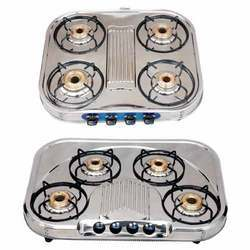
\includegraphics{images/4-burner.jpg}\\
\end{center}

\end{changemargin}
\end{frame}


\begin{frame}
\frametitle{The Human Factor: USB Cables}
\begin{changemargin}{1cm}

\vspace{-0.5em}
\begin{center}
	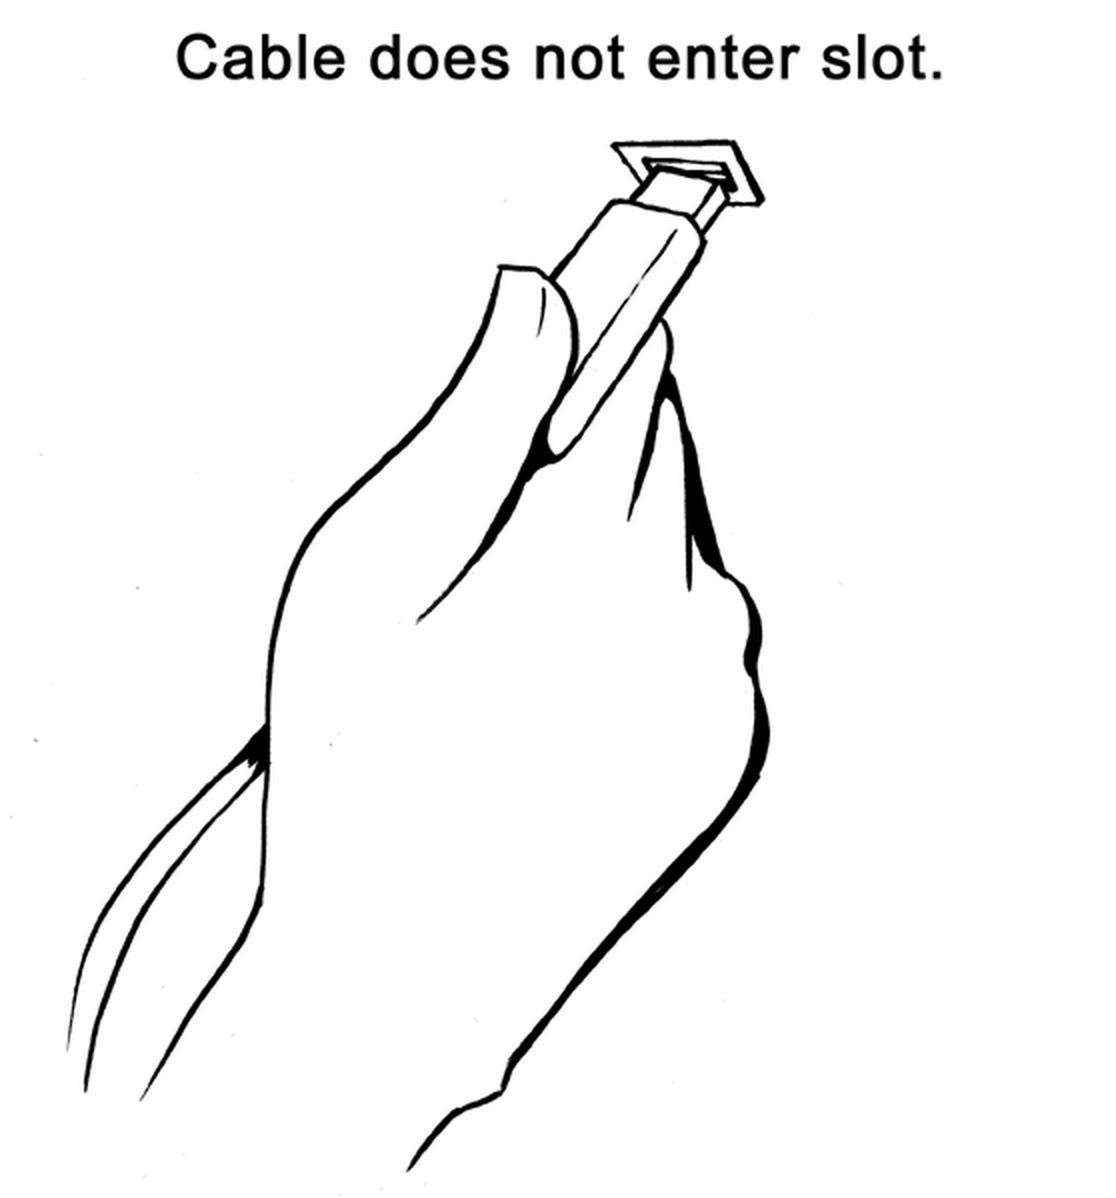
\includegraphics[height=20em]{images/usb1.png}\\
\end{center}

\end{changemargin}
\end{frame}

\begin{frame}
\frametitle{The Human Factor: USB Cables}
\begin{changemargin}{1cm}

\vspace{-0.5em}
\begin{center}
	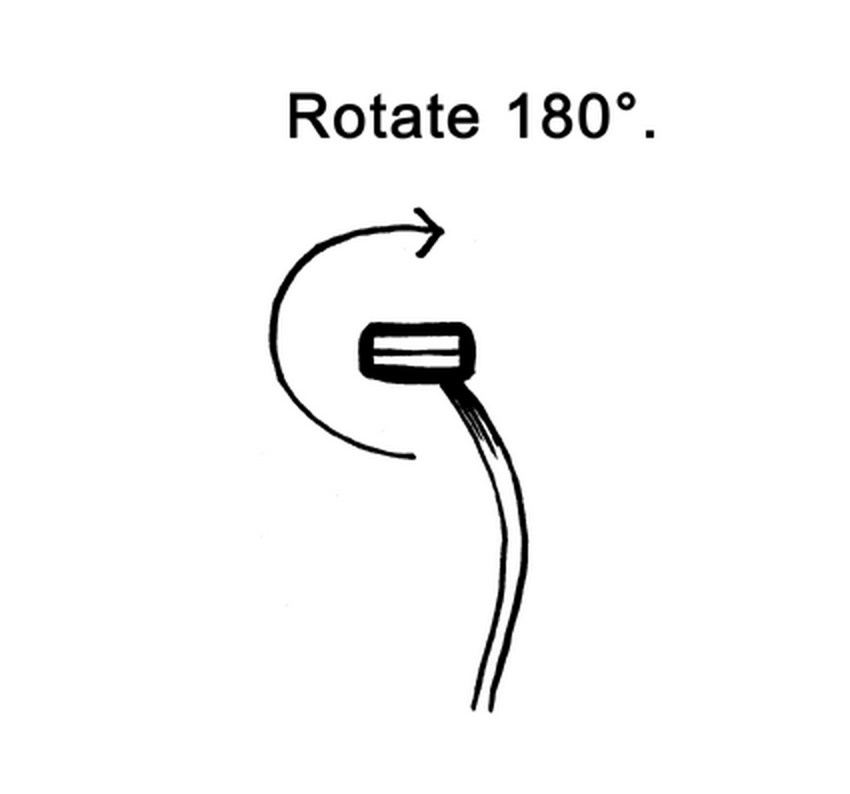
\includegraphics[height=20em]{images/usb2.png}\\
\end{center}

\end{changemargin}
\end{frame}


\begin{frame}
\frametitle{The Human Factor: USB Cables}
\begin{changemargin}{1cm}

\vspace{-0.5em}
\begin{center}
	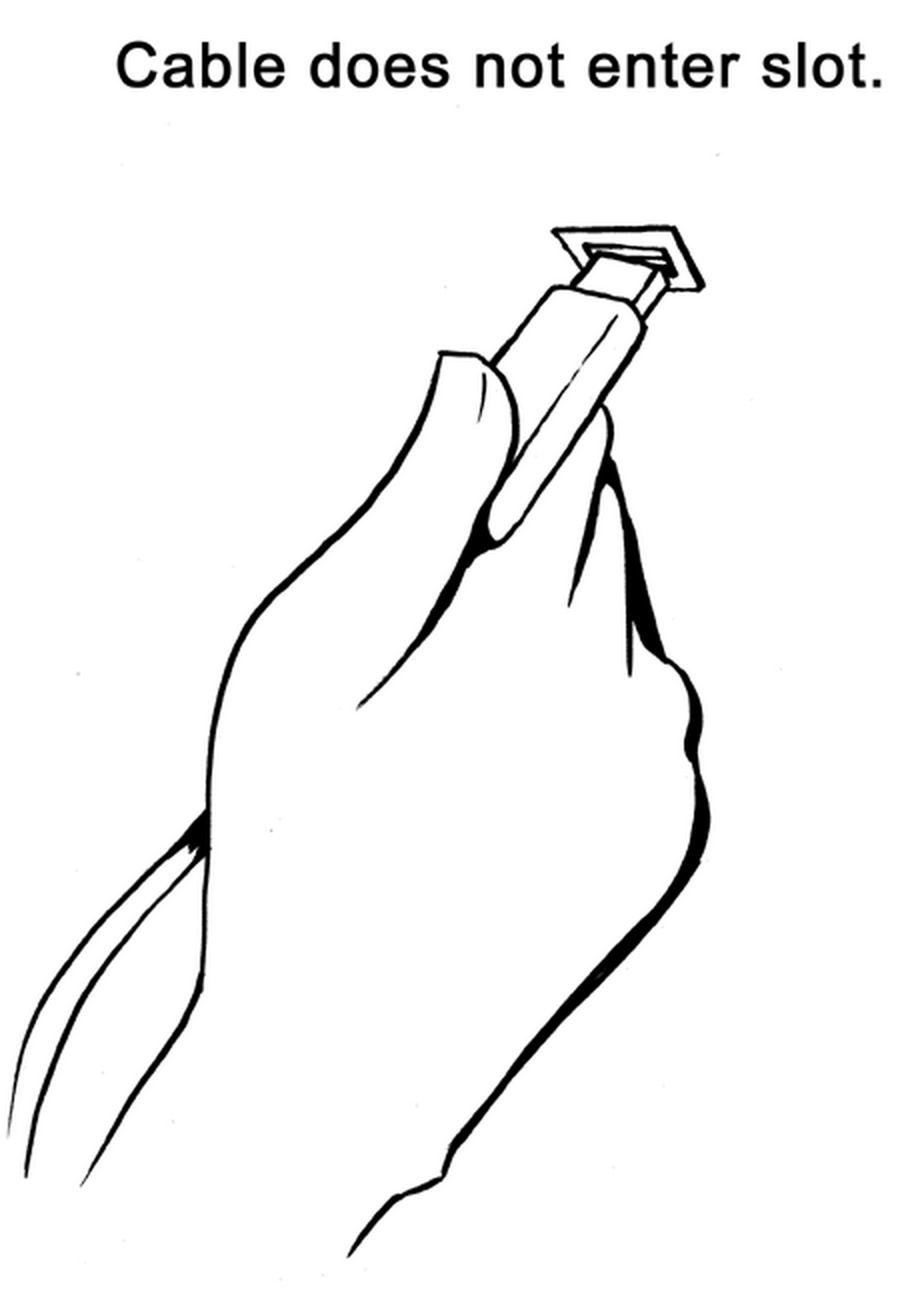
\includegraphics[height=20em]{images/usb3.png}\\
\end{center}

\end{changemargin}
\end{frame}


\begin{frame}
\frametitle{The Human Factor: USB Cables}
\begin{changemargin}{1cm}

\vspace{-0.5em}
\begin{center}
	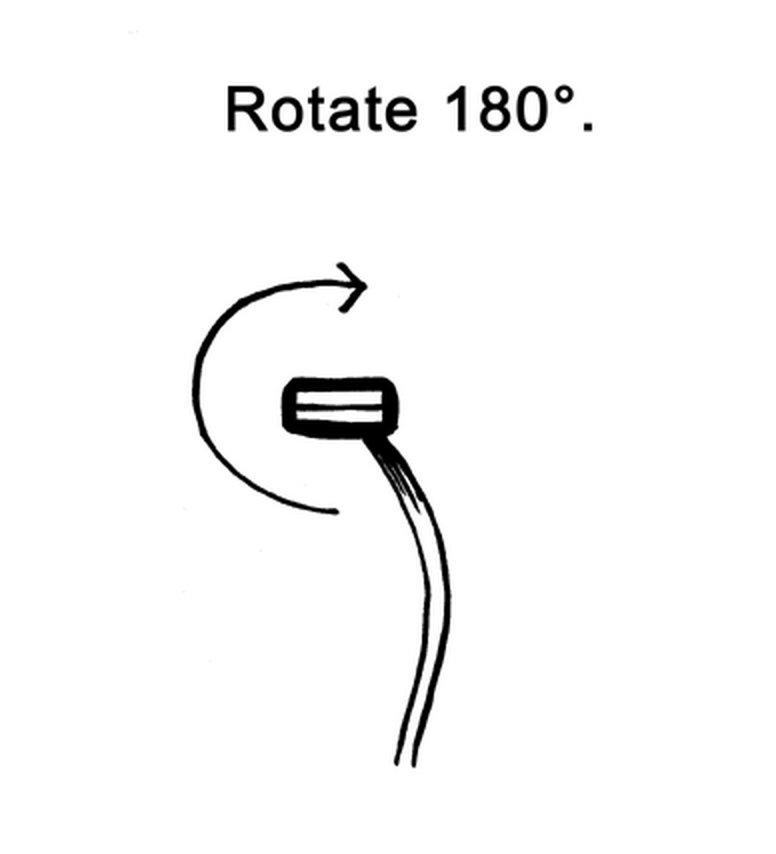
\includegraphics[height=20em]{images/usb4.png}\\
\end{center}

\end{changemargin}
\end{frame}


\begin{frame}
\frametitle{The Human Factor: USB Cables}
\begin{changemargin}{1cm}

\vspace{-0.5em}
\begin{center}
	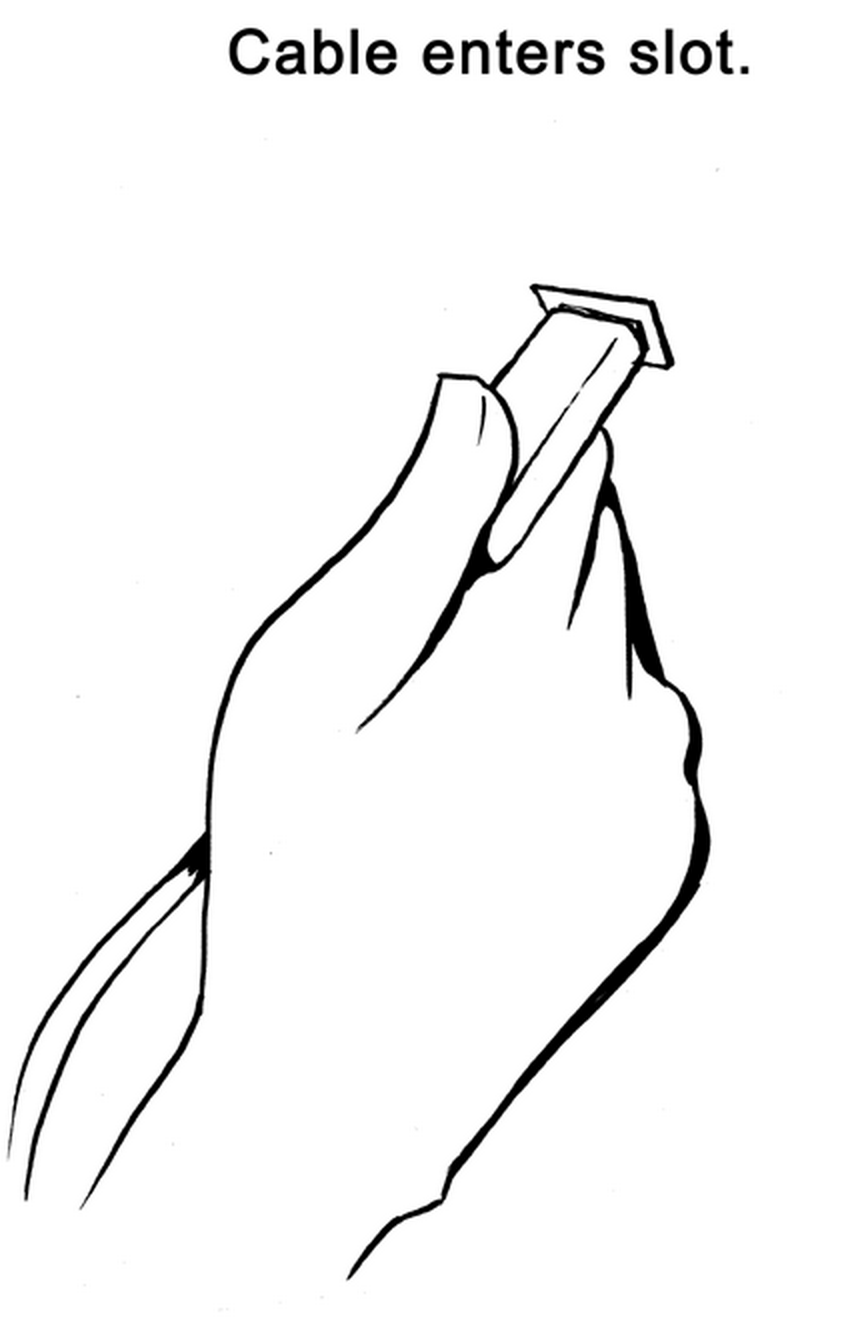
\includegraphics[height=20em]{images/usb5.png}\\
\end{center}

\end{changemargin}
\end{frame}


\begin{frame}
\frametitle{The Human Factor: Make Errors Impossible}
\begin{changemargin}{1cm}

[USB pictures from \texttt{http://www.smbc-comics.com/?id=2388}.]

USB group has finally figured it out:\\
\quad Type C connector is reversible. No ``wrong'' way.

Or laptop batteries: asymmetrical, obvious how it fits in.

\end{changemargin}
\end{frame}


\begin{frame}
\frametitle{The Human Factor: Feedback}
\begin{changemargin}{1cm}

Humans respond well to feedback.

Imagine a campfire. \mnote{If you try to get too close, the temperature increases until it feels uncomfortable, and if you get really close it can get painful. When you step away, the temperature decreases.}

It's obvious what happens if you step towards/away from fire.

Warning signs: discomfort or pain to warn of the danger of getting too close (getting burned).

\end{changemargin}
\end{frame}

\begin{frame}
\frametitle{The Human Factor: Feedback}
\begin{changemargin}{1cm}
Lack of feedback results in a lot of errors.

Not sure if button press worked? Press again.

Did that send it twice?

Example: TV with a slow turn-on. \mnote{or example, my grandmother's flat screen TV. When you press the power on the remote, it takes a few seconds before any indication appears on the TV that it's powering on (a little LED comes on). The result is that for the first few seconds, I don't know if I pressed the power button while the remote had proper line of sight to the receiver successfully or not. If it was but I think it wasn't, I press the button again. This results in the TV turning on briefly before turning off. Or if my command hadn't been received I might sit there for a few seconds before I realize I need to press the button again. On most TVs, including mine, as soon as I press the power button, a little LED lights up in the corner (and I hear a click) to tell me it's turning on.}

\end{changemargin}
\end{frame}

\begin{frame}
\frametitle{The Human Factor: Feedback and Safety Rules}
\begin{changemargin}{1cm}
\begin{quote}
\textit{Breaking safety rules is usually reinforced, which is to say, it pays off. Its immediate consequence is only that the violator is rid of the encumbrance the rules impose and can act more freely. Safety rules are usually devised in such a way that a violator will not immediately be blown sky high, injured, or harmed in any other way, but will instead find that his life is made easier... The positive consequences of of violating safety rules reinforce our tendency to violate them, so the likelihood of a disaster increases.}
\end{quote}
\hfill Dietrich D\"orner

\mnote{This tendency cannot be ignored in the design of systems, especially safety-critical ones. The feedback we receive from breaking the safety rules is dangerous.}

\end{changemargin}
\end{frame}


\begin{frame}
\frametitle{The Human Factor: Conclusion}
\begin{changemargin}{1cm}

We require UW Eng students to take a class in economics.

It doesn't make anyone an expert in economics;\\
\quad It exposes students to the relevance of economic factors.

Engineering projects will eventually involve interaction between technologies and humans.

Brief introduction to the human factor is the least we can do.

\end{changemargin}
\end{frame}

\end{document}
